\documentclass{beamer}

\usepackage{graphicx}
\usepackage{listings}

\title{Apresentação sobre o BattleShips}
\author{Daniel Rosso Strutz}

\begin{document}
\maketitle
 
\begin{frame}

\frametitle{raylib}
 
\begin{figure}[h]
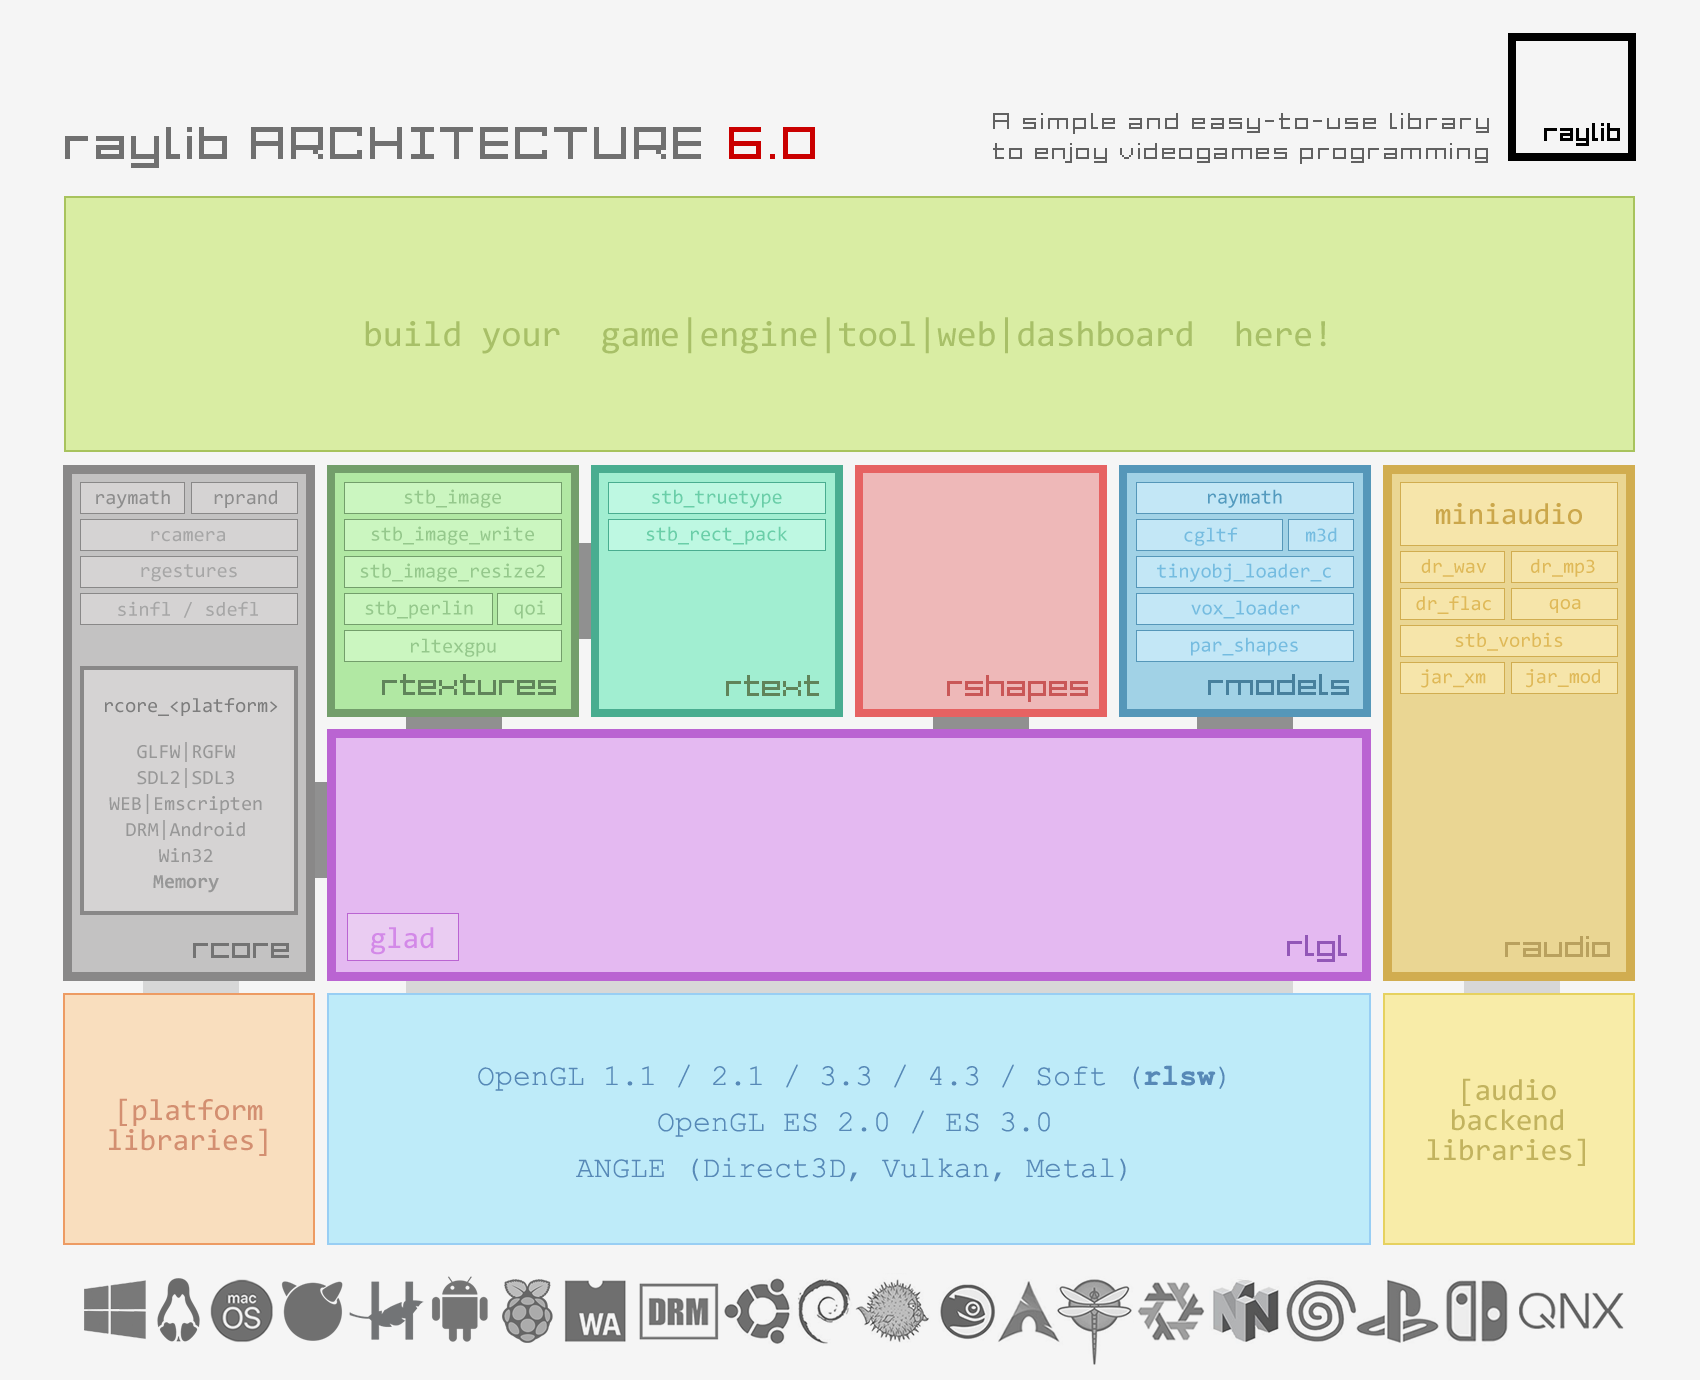
\includegraphics[width=10cm]{raylibArch.png}
\end{figure}
 
\end{frame}

\begin{frame}
 
\frametitle{rayalarm}
 
\begin{figure}[h]
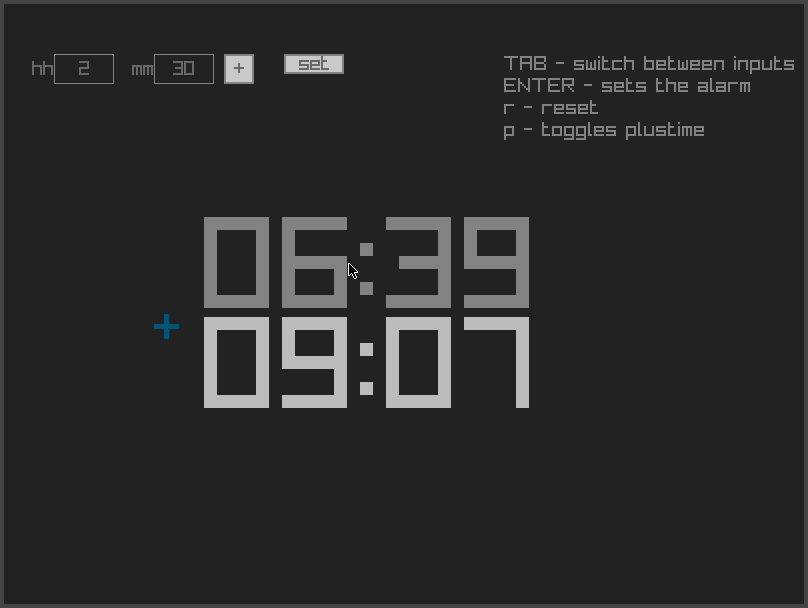
\includegraphics[width=10cm]{rayalarm.png} 
\end{figure}
 
\end{frame}

\begin{frame}[fragile]
 
\frametitle{Um retângulo:}

\begin{lstlisting}[language=c++, basicstyle=\small]
Vector2 posicao = {
    .x = 10,
    .y = 20,
};

Rectangle exemplo = {
    .x = posicao.x,
    .y = posicao.y,
    .width = 100, 
    .height = 200, 
};

DrawRectangleRec(exemplo, BLUE); 
\end{lstlisting}

\end{frame}
 
\begin{frame}[fragile]
\frametitle{A história toda:}
\begin{lstlisting}[language=c++, basicstyle=\tiny]
#include "raylib.h"

int main (){ 
     
    InitWindow(800, 600, "rect");
    SetTargetFPS(60);
     
     
    while(!WindowShouldClose()){ 
    BeginDrawing(); 
     
    Vector2 posicao = {
        .x = 10,
        .y = 20,
    };

    Rectangle exemplo = {
        .x = posicao.x,
        .y = posicao.y,
        .width = 100, 
        .height = 200, 
    };
     
    DrawRectangleRec(exemplo, BLUE); 
     
    EndDrawing();
    }

    CloseWindow();
}
\end{lstlisting}
 
\end{frame}
 
\begin{frame}
\frametitle{E o resultado:}

\begin{figure}[h]
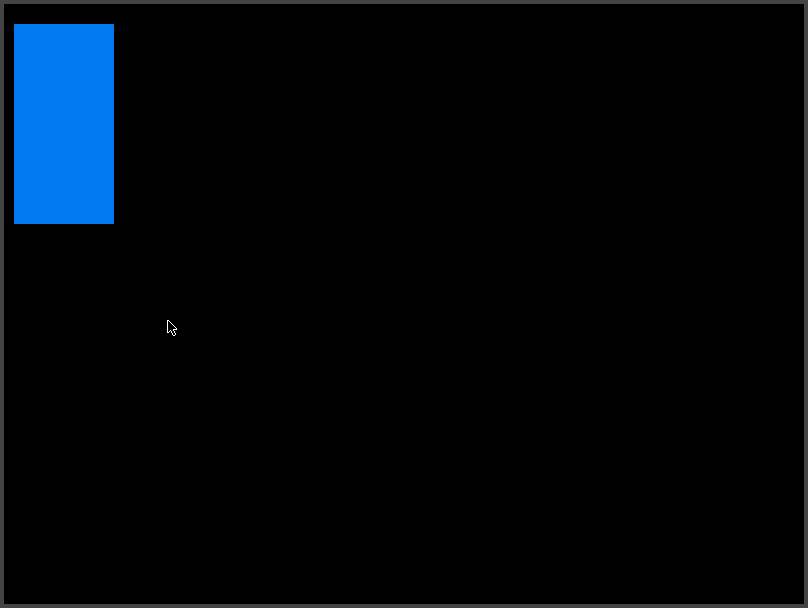
\includegraphics[width=10cm]{rectExemplo.png}
\end{figure}

\end{frame}

\begin{frame}
\frametitle{Extrapolando o conceito:}

\begin{figure}[h]
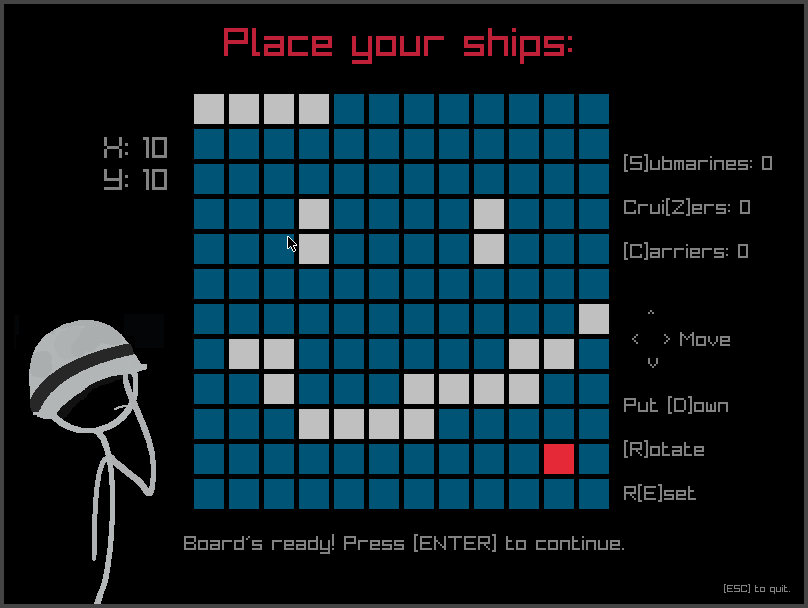
\includegraphics[width=10cm]{placeships.png}
\end{figure}

\end{frame}

\begin{frame}
\frametitle{Tudo de novo igual, só que diferente:}
 
\begin{figure}[h]
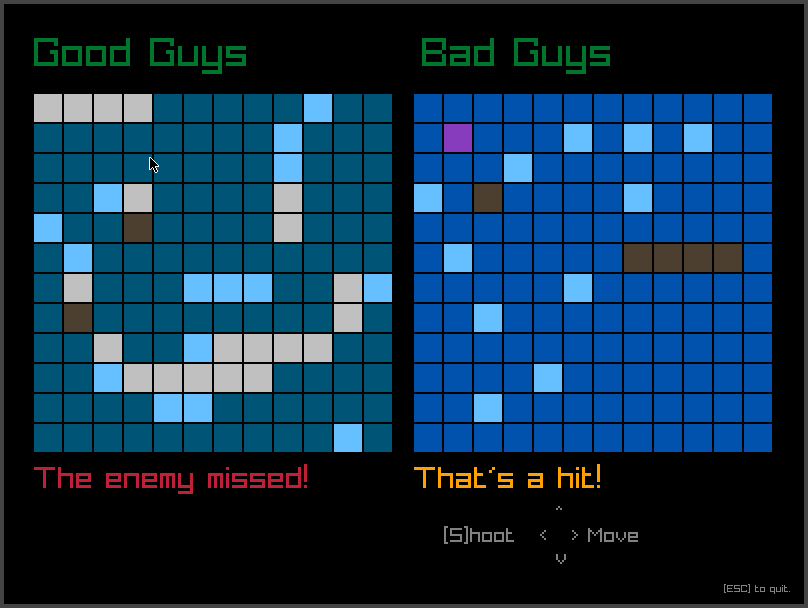
\includegraphics[width=10cm]{battle.png}
\end{figure}
 
\end{frame}

\begin{frame}
\frametitle{Recursos utilizados}
\begin{enumerate}
 
\item Pacotes do {\LaTeX}:
 
\begin{itemize}
\item beamer
\item graphicx
\item listings
\end{itemize}
 
\item https://www.raylib.com/examples.html
 
\end{enumerate}
 
\bigbreak
\centerline{\textbf{https://github.com/danirosso}}
 
\end{frame} 
 
\end{document}
